
%****************************************************
%\section{Framework introduction}
%\label{Intro_nemico}
%****************************************************
%This Chapter of the dissertation will introduce a big data mining framework in which distributed frequent itemset mining algorithms are just one of the possible tools or modules. While in this Chapter the framework will be briefly introduced, in Chapter \ref{mgi}, two use cases of the framework will be evaluated, in which FIM algorithms are leveraged  to mine new type of itemsets. 

This Chapter of the dissertation will introduce (i) a big data mining framework and (ii) its utilization to extract a new type of itemsets, called misleading generalized itemsets.
The comprehensive framework was initially designed to analyze network traffic logs (textbf{to do: add citazione nemico}) and provide users with a variety of network analytics services. After that, it has been extended to support a new real life scenario (Smart Cities environment) and to focus on a new type of itemset called misleading generalized itemsets {to do: add citazione mgi e mgi polito madrid}
The first use case taken into account to evaluate the effectiveness of the framework is related to network traffic analysis. In this field, important issues are communication profiling, anomaly or security threat detection, and recurrent pattern discovery.  
Traffic analyses are commonly performed on: (i) packet payloads, (ii) traffic metrics, or (iii) some statistical features computed on traffic flows. 
In the second use case, the proposed framework has been applied to analyze the traffic law infractions committed by 
the citizens of Turin, an important business and cultural center in northern Italy. 
Real infraction data is provided as open data by the Turin administration.
The target of the analysis is to improve the efficiency of public services, 
the transparency of public administrations, and the awareness of the degree of civilization of urban people.

Especially for network traffic analysis, a significant research effort has been devoted to the application of data mining techniques. The proposed approaches address
the discovery of significant correlations among data~\cite{NostroComNet,EGI}, the extraction of knowledge useful for prediction~\cite{KaragiannisPF05}, and 
the clustering of network data with similar properties~\cite{Erman05}.
However, due to the continuous growth in network speed, petabytes of data may be transferred through a network every day. 
These ''big data'' collections stress the limits of existing data mining techniques and thus they set new horizons for the design of innovative data mining approaches.
%
%The goal of the proposed work is the design and the development of a comprehensive system which provides users with a variety of network analytics services. 

The Chapter is organized as follows. Section~\ref{arch} presents \Nemico\ (\NemicoDef), a data mining system focused on efficiently discovering interesting knowledge from Big network datasets by means of distributed approaches.
After that, in Section~\ref{mgi_intro}, we will introduce an instance of the framework, named \SeTAB\ (\SeTA ), developed to mine misleading generalized itemsets.
%, and evaluate its performance in two real life scenarios related to network traffic and law infractions.
Section~\ref{relwork} overviews most relevant previous works while Section~\ref{probstat} states the problem addressed in this
work. Section~\ref{setarch} presents the \SeTAB\ architecture while an experimental evaluation of our approach is reported in Section~\ref{exp}. Finally,
Section~\ref{conclusion} draws conclusions and discusses future research directions.


%****************************************************
\section{The \Nemico\ architecture}
\label{arch}
%****************************************************
\Nemico\ consists of a series of distributed MapReduce jobs related to different step of the knowledge discovery process. It ranges from network data acquisition to knowledge exploitation, as we will detail in the next chapters. 
In Figure~\ref{fig:arch} are shown the building blocks of the \Nemico\ architecture.
%The system has been thought to support the integration of a variety of data mining algorithms, including supervised approaches (e.g., classification and regression algorithms) and unsupervised ones (e.g., association rule mining, clustering).
To effectively support analysts in discovering different and interesting kinds of knowledge, a broad variety of data mining algorithms can be integrated in the system such as exploratory techniques (e.g., association rules, clustering) and prediction ones (e.g., classification and regression algorithms). 

In this job pipeline, each job takes as input the result of one or more preceding jobs, performing a specific step of the data mining process.
(each job is performed by one or more MapReduce tasks running on a Hadoop cluster).


\begin{figure}
\centering
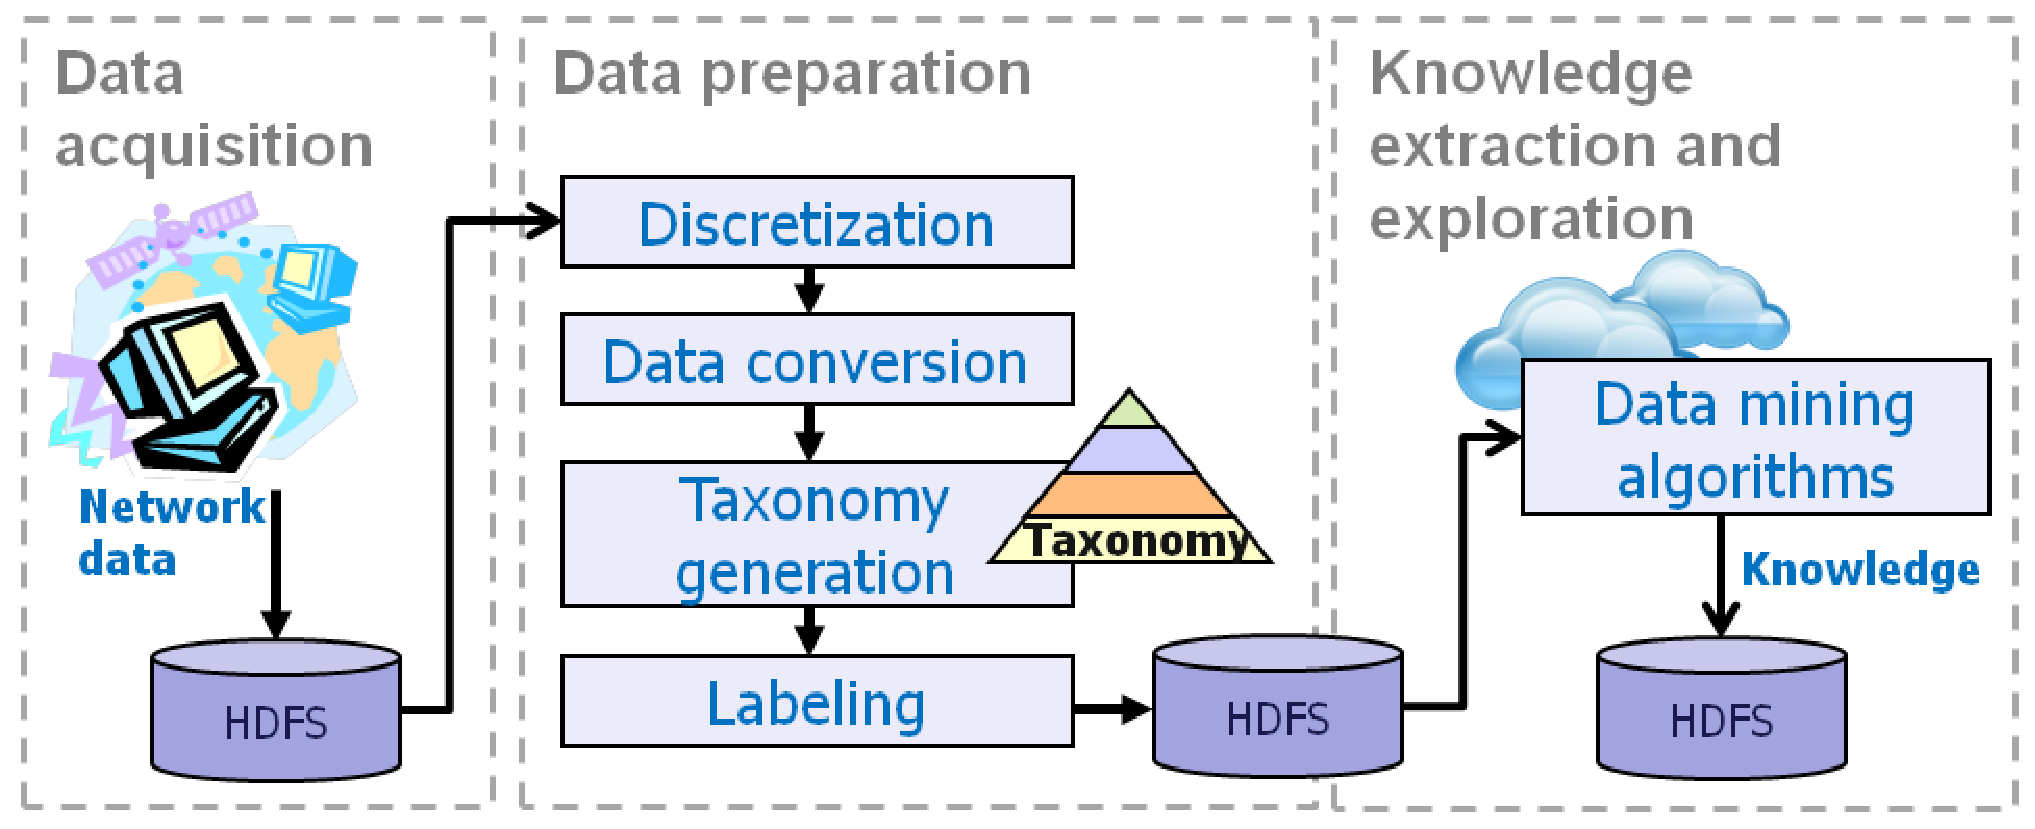
\includegraphics[width=1\textwidth]{chapters/nemico/Framework.eps}
\caption{Architecture of \Nemico}
\label{fig:arch}
\end{figure}



%****************************************************
\subsection{Data acquisition and preprocessing}
\label{Netacq}
%****************************************************

\Nemico\ exploits passive traffic sniffing to acquire massive amounts of network traffic measurements and stores them in HDFS distributed file system.
%A passive probe located on the Internet access link of an edge network is exploited to acquire incoming and outgoing packets flowing on the link. 
More details about the specific use case data preparation will be provided in Section \textbf{to add}.
%Traffic monitoring is performed by Tstat~\cite{Tstat}, a tool that allows users to collect network and transport layer measurements. 
%%Tstat rebuilds TCP connections by matching sequence numbers on data segments with the corresponding acknowledgement (ACK) numbers.
%The acquired datasets consist of a set of records, each one corresponding to a different TCP flow.
%To ensure measurement reliability, only the TCP flows that last more than ten packets (i.e., the long-lived flows) are considered.
%
%\Nemico\ stores the collected network traffic data in an HDFS distributed file
%system.  It can successfully acquire and handle all the network measurements provided by Tstat (i.e., the Round-Trip-Time (RTT) observed on a TCP flow, the class of application layer service (e.g., HTTP,VIDEO) assigned by Tstat). 

%Among others, the supported measurements comprise (i) the Round-Trip-Time (RTT) observed on a TCP flow, which indicates the minimum time lag between the observation of a TCP segment and the observation of the corresponding ACK, (ii) the TCP port of the server, (iii) the number of packets, and (iv) the class of application layer service (e.g., HTTP,VIDEO) assigned by Tstat. Note that Tstat measurements comprise both continuous values (e.g., the RTT) and discrete values (e.g., the class of service).  

%%****************************************************
%\subsection{Data preparation}
%\label{dataprep}
%%****************************************************

To suit the raw data to each of the subsequent data mining step, are applied some data preprocessing steps to the input data.
A brief description of the main data preparation steps is given below.

\textbf{Discretization}. Discretization concerns the transformation of continuous values into discrete ones. Since some data mining algorithms are unable to cope with continuously valued data, 
measurement values are discretized prior to running the algorithms. 
%In some cases (e.g., the association rule mining algorithms) discretization is not mandatory but strongly recommended because considering continuously valued attributes could bias the mining result (e.g., the association rules extracted from continuously valued attributes are unlikely to occur frequently in the source data). 
The discretization step can be performed either automatically by using established techniques~\cite{libroKumar} or semi-automatically by partitioning continuous value ranges into appropriate bins based on the prior knowledge about the measurement domains. 
%Due to the nature of the analyzed network data, manual data discretization is commonly preferable.  

\textbf{Data conversion}. Data conversion entails the transformation of the raw data into the data format expected by the data mining algorithms to apply. It happens that algorithms are designed to handle only a subset of specific format. For example, most association rule mining algorithms are designed to cope with transactional data~\cite{libroKumar}. Hence, applying association rule mining algorithms requires the acquired data to be tailored to the transactional data format. 

\textbf{Taxonomy generation}. The data mining process can be driven by semantics-based models (e.g., taxonomies or ontologies). These models, when available, are used to enrich the source data with multiple-level or multi-faceted information that would result in additional knowledge as output.  
For instance, a taxonomy, as shown in this Chapter for the use-cases taken into account, consists of set of 'is-a' hierarchies built over the data attributes. These structures are exploited to aggregate specific data values (e.g., the TCP ports) into meaningful higher-level categories.
\Nemico\ supports both
the automatic taxonomy inference over a subset of specific network data attributes (e.g., port number, packet number) 
and the semi-automatic taxonomy construction. 
%The mining process for extracting more abstract and interesting correlations among data (e.g., generalized association rules) is driven by taxonomies. 
%A taxonomy is a hierarchy of aggregations over values of one attribute (e.g., TCP port) and it is usually represented as a tree. 
%\Nemico\ allows either to automatically infer interesting taxonomies directly from the data. 
%To this aim different algorithms have been devised and implemented to automatically extract taxonomies for the considered attributes (i.e., port number, packet number) since some attributes (e.g., port number) are actually hierarchical attributes while others are numerical ones.
%In \Nemico\ taxonomies could also be provided directly by the user.

\textbf{Labeling}. Supervised data mining techniques (e.g., classification) require the labeling of one data attribute 
as class label. Hence, if the data mining process comprises supervised analyses domain-experts have to specify the class attribute. 


The current implementation of \Nemico\ includes a first implementation of all the described activities as parallel map jobs.



\comment{The current implementation of \Nemico\ includes the implementation of both data discretization and conversion which are performed by a single map only job. Each record is processed by the map
function and, if the number of packets is above the threshold (e.g., 10 packets), the corresponding discretized version is generated as output of the mapping step.
This task entails an inherently parallel elaboration, considering that can be applied independently to each record.}



%****************************************************
\subsection{Knowledge extraction and exploration}
\label{KnowExt}
%****************************************************
Knowledge extraction entails the application of data mining algorithms to find implicit, previously unknown, and potentially useful information from large volumes of network data. 
\Nemico\ comprises novel data mining algorithms that contribute to a paradigm-shift in distributed data mining. The analytics algorithms entail (i) discovering underlying correlations among traffic data 
(e.g., multiple-level associations among data equipped with taxonomies), (ii) grouping traffic flows with similar properties (e.g., clustering), and (iii) extracting models useful for prediction (e.g., classification, regression).  
%The algorithms are designed to address the following issues.
%
%\textit{Sparse data distribution.} Since Big data collections have large cardinality and/or a high number of dimensions, they are usually characterized by an
%inherent sparseness. Aimed at addressing this issue, we propose incremental algorithms that are able to cope with result refinement over different incremental runs
%and that scale by adapting to new data without the need for re-analyzing the entire dataset.
%
%\textit{Algorithm optimization}. Most data mining algorithms are poorly optimized for cloud computing environments. 
%Conversely, our algorithms have specifically been designed to scale %improve the scalability of the existing techniques and their performance 
%in massively parallel computing environments.
%
%\textit{Horizontal scalability.} To apply the data mining techniques to petabyte-scale network traffic datasets, \Nemico\ integrates advanced analytics algorithms (e.g., association rule mining) with horizontally scalable approaches, 
%such as those based on Map Reduce and shared columnar storage backends.

As already mentioned, the current implementation of \Nemico\ comprises Hadoop-based data mining algorithms focused on the extraction of interesting and multiple-level correlations among network data (~\cite{ISPA14}). The next Section will describe the application of such comprehensive framework to the Network traffic and Smart Cities environments.

%**********************************************************
%\subsection{Knowledge categorization and selection}
%\label{KnowCatSel}
%**********************************************************
%Explorative data mining approaches, such as association rule mining and clustering algorithms, may identify interesting knowledge, which may be both huge in size and complex in structure. To ease exploitation of the mined knowledge, different
%interestingness measures (e.g., chi square, support expectation, collective strength) to reduce and evaluate the amount of extracted knowledge  are  needed. For a detailed review on measures for interesting rules and quality indexes for clustering see \cite{Hilderman2001} and  \cite{KumarBook} respectively. The current implementation of \Nemico\ includes COSA METTIAMO??

%Furthermore, only for the discovery of correlations when coping with relatively
%large or complex transactional network datasets the number of mined rules could be
%so large that a manual inspection becomes unfeasible. To overcome this issue, \Nemico\ propose a classification of the rules into
%groups according to their semantics in the network domain. 
%
%%**********************************************************
%\section{Experiments and conclusions}
%\label{conc}
%%**********************************************************
%
%The current implementation of \Nemico\ was developed in Java using the Hadoop Java APIs. It was validated on real network traffic datasets with size 192.56 GB. The experiments were performed on a cluster of 5 nodes running the Cloudera's
%Distribution of Apache Hadoop (CDH4.5). More details of both cluster node and data can be found in \cite{ISPA14}. 
%For both data mining algorithms in \Nemico , we evaluated the speedup achieved increasing the number of Hadoop cluster nodes and the achieved results show that our approaches scale roughly linearly with the number of nodes and the speedup approximately
%corresponds to the number of cluster nodes. As future work we are planning to introduce visualization tools and new data mining algorithms to support
%a larger variety of traffic data analyses. 

